\documentclass[openright,twoside,10pt]{memoir}
%
% Packages
%
%\usepackage[utf8]{inputenc}
\usepackage[T1]{fontenc}
\usepackage[danish]{babel}
\linespread{1.05}
\usepackage{fontspec}

\setmainfont[Ligatures=TeX]{Garamond}
\setmonofont{Consolas}

% Eksempel
%\newfontfamily{\titlefont}{Antique-Olive Th}

%\newcommand{\heading}[1]{ \vspace{0.5cm} {\titlefont \Large #1}\\ }
%\newcommand{\bilagtitle}[1]{ {\titlefont \LARGE #1}\\ }

%---- 

\usepackage{tocloft}
\usepackage[toc]{multitoc}

\renewcommand*{\multicolumntoc}{2}

\chapterstyle{hangnum}
\raggedbottom
\setlength{\beforechapskip}{0pt}
\setlength{\afterchapskip}{10pt} % vspace under chapters
\setlength{\belowcaptionskip}{-7pt} % vspace mellem caption og tekst
\setlength{\cftparskip}{3pt}
\setlength{\cftbeforechapterskip}{7pt}
\setlength{\cftbeforepartskip}{14pt}
\setsecnumdepth{subsection}

\renewcommand*{\partnamefont}{\normalfont\Huge\bfseries}
\renewcommand*{\partnumfont}{\normalfont\Huge\bfseries}
\renewcommand*{\parttitlefont}{\normalfont\HUGE\bfseries}
\renewcommand*{\chaptitlefont}{\normalfont\HUGE\bfseries}
\setsecheadstyle{\normalfont\huge\bfseries}
\setsubsecheadstyle{\normalfont\Large\bfseries}
\setsubsubsecheadstyle{\normalfont\large\bfseries}

%% Fonts
%\usepackage[sc]{mathpazo}
%\usepackage{courier}
%\usepackage{inconsolata}
%\usepackage[scaled]{uarial}
%\renewcommand*\familydefault{\sfdefault}

% En pil...
\usepackage{textcomp}

\usepackage{multirow}
\usepackage{tabularx}
\usepackage{icomma}
\usepackage{amsmath,amsfonts,amssymb}
\usepackage{mathtools}
\usepackage{graphicx}
\usepackage{gensymb}
\usepackage[usenames,dvipsnames,table]{xcolor} % til farvning af celler i tabel
\usepackage{url}
%\usepackage[bottom]{footmisc} % keep footnotes at bottom UNCOMMENTED
%PGA errors
\usepackage{bbding}
\usepackage{pdfpages}
\usepackage{float} %kan bruge H placement modifier, bedre end "h!"
%\usepackage{wrapfig}
\usepackage{subfig}
%\usepackage{sagetex}
\usepackage[section]{placeins}
\usepackage{xspace}
\usepackage[chapter]{algorithm}
\usepackage{algpseudocode}
\usepackage{algorithmicx}

\parskip=5pt plus 2pt minus 1pt
\parindent=0pt
\frenchspacing % kommeretninger

% Fancy ting med enheder og datatabeller. Læs manualen til pakken
% Manual: http://www.ctan.org/tex-archive/macros/latex/contrib/siunitx/siunitx.pdf
\usepackage{siunitx}

%\usepackage{siunitx}
%\usetikzlibrary{shapes}
\usepackage{enumitem} %stackoverflow.com/questions/3275622/latex-remove-spaces-between-items-in-list
\usepackage{listings}
%\setcounter{secnumdepth}{3}
%\setcounter{tocdepth}{3}

\definecolor{shcomment}{rgb}{0.12, 0.38, 0.18 }
%adjusted, in Eclipse: {0.25, 0.42, 0.30 } = #3F6A4D
\definecolor{shkeyword}{rgb}{0.37, 0.08, 0.25}  % #5F1441
\definecolor{shstring}{rgb}{0.06, 0.10, 0.98} % #101AF9
\definecolor{fpcolor}{rgb}{0.13, 0.31, 0.09} % #101AF9

\setfloatlocations{figure}{htb}

 \lstset{ % http://stackoverflow.com/questions/741985/latex-source-code-listing-like-in-professional-books
%         basicstyle=\footnotesize\ttfamily,% the size of the fonts
                                % that are used for the code
        basicstyle=\footnotesize\ttfamily,% the size of the fonts that are used for the code
         numbers=left,                     % where to put the line-numbers
         numberstyle=\tiny,                % the size of the fonts that are used for the line-numbers
         stepnumber=1,                     % line numbering steps
         numbersep=5pt,                    % how far the line-numbers are from the code
         tabsize=2,                        % sets default tabsize to 2 spaces
         breaklines=true,                  % sets automatic line breaking
         keywordstyle=\color{shkeyword},        % language function text color
    		frame=b,
 %        keywordstyle=[1]\textbf,    % Stil der Keywords
 %        keywordstyle=[2]\textbf,    %
 %        keywordstyle=[3]\textbf,    %
 %        keywordstyle=[4]\textbf,   \sqrt{\sqrt{}} %
         stringstyle=\color{shstring}, % string text color
%         stringstyle=\color{red},
        commentstyle=\color{shcomment},
         showspaces=false,           % show spaces adding particular underscores
         showtabs=false,             % show tabs within strings adding particular underscores   
         showstringspaces=false,     % underline spaces within strings
         xleftmargin=17pt,
         framexleftmargin=17pt,
         framexrightmargin=5pt,
         framexbottommargin=4pt,
         language=Ruby
 }
    %\DeclareCaptionFont{blue}{\color{blue}} 

%\captionsetup[lstlisting]{singlelinecheck=false, labelfont={blue}, textfont={blue}}
\DeclareCaptionFont{white}{\color{white}}
\DeclareCaptionFormat{listing}{\hrule\smallskip\parbox{\textwidth}{\hspace{15pt}#1#2#3}\smallskip\hrule}
\captionsetup[lstlisting]{format=listing,
  singlelinecheck=false, margin=0pt, font={bf,footnotesize}}

\usepackage{tocvsec2}


\usepackage{memhfixc}
%
% Fra AAU temp
%
\usepackage{calc}
\usepackage{lastpage}

\usepackage{hyperref}
%
% Layout
%
\newenvironment{indledning}{\sffamily}{\vskip 0.75cm}
\newenvironment{tail}{\vskip 0.75cm\itshape}{}
\newcommand{\spc}[1] {#1 \vskip 1cm}
\definecolor{aaublue}{HTML}{0492D2}

\let\oldmarginpar\marginpar
\renewcommand\marginpar[1]{\-\oldmarginpar[\raggedleft\footnotesize #1]%
{\raggedright\footnotesize\color{red} #1}}
% Margins
\setstocksize{11in}{8.5in}
\settrimmedsize{11in}{8.5in}{*}
\settrims{0in}{0in}
\settypeblocksize{9.0in}{6in}{*}
\setlrmargins{1.25in}{*}{*}
\setulmargins{1.0in}{*}{*}
\setheadfoot{14pt}{26pt}
\setheaderspaces{*}{13pt}{*}

% Fra settings.tex
\setlrmarginsandblock{3.5cm}{2.5cm}{*}
\setulmarginsandblock{2.5cm}{3.0cm}{*}

\checkandfixthelayout
%
% Tikz
%
%\tikzstyle{block}=[draw, rectangle, text width=2cm, minimum height=1cm, text badly centered, node distance=\afs]
%\tikzstyle{cloud}=[draw, ellipse, minimum width=2cm, fill=gray!40]
%\tikzstyle{valg} = [draw, diamond, inner sep=1pt, text badly centered, text width=4.5em]
%\tikzstyle{pil} = [draw, -latex]

\setlength{\unitlength}{2em} % for the picture environment

\usepackage[compact]{titlesec}
\titlespacing{\section}{0pt}{*0}{*0}
\titlespacing{\subsection}{0pt}{*0}{*0}
\titlespacing{\subsubsection}{0pt}{*0}{*0}

% Forhindrer horeunger..:

\widowpenalty=300
\clubpenalty=300

\setlength{\parskip}{3ex plus 2ex minus 2ex}

%extra colonner til titelbladet
\usepackage{multicol}

% procenttegn
\let\oldpercent=\%
\renewcommand{\%}{\ifmmode\ \oldpercent\else\oldpercent\fi}

%
% Check-in by Niels on November 07
%
% Alter some LaTeX defaults for better treatment of figures:
    % See p.105 of "TeX Unbound" for suggested values.
    % See pp. 199-200 of Lamport's "LaTeX" book for details.
    %   General parameters, for ALL pages:
    \renewcommand{\topfraction}{0.9}	% max fraction of floats at top
    \renewcommand{\bottomfraction}{0.8}	% max fraction of floats at bottom
    %   Parameters for TEXT pages (not float pages):
    \setcounter{topnumber}{2}
    \setcounter{bottomnumber}{2}
    \setcounter{totalnumber}{4}     % 2 may work better
    \setcounter{dbltopnumber}{2}    % for 2-column pages
    \renewcommand{\dbltopfraction}{0.9}	% fit big float above 2-col. text
    \renewcommand{\textfraction}{0.07}	% allow minimal text w. figs
    %   Parameters for FLOAT pages (not text pages):
    \renewcommand{\floatpagefraction}{0.7}	% require fuller float pages
	% N.B.: floatpagefraction MUST be less than topfraction !!
    \renewcommand{\dblfloatpagefraction}{0.7}	% require fuller float pages


%
% Weird shit added by Niels on December 13
% Changes style of bibliography
%
\makeatletter
\renewenvironment{thebibliography}[1]
     {\chapter*{\bibname}
     \addcontentsline{toc}{part}{\bibname}
      \@mkboth{\MakeUppercase\bibname}{\MakeUppercase\bibname}%
      \list{\@biblabel{\@arabic\c@enumiv}}%
           {\settowidth\labelwidth{\@biblabel{#1}}%
            \leftmargin\labelwidth
            \advance\leftmargin\labelsep
            \@openbib@code
            \usecounter{enumiv}%
            \let\p@enumiv\@empty
            \renewcommand\theenumiv{\@arabic\c@enumiv}}%
      \sloppy
      \clubpenalty4000
      \@clubpenalty \clubpenalty
      \widowpenalty4000%
      \sfcode`\.\@m}
     {\def\@noitemerr
       {\@latex@warning{Empty `thebibliography' environment}}%
      \endlist}
\makeatother

% Degrees
%\newcommand{\degree}{\ensuremath{^\circ}}
\DeclareMathOperator*{\argmax}{arg\,max}


% References
\newcommand{\secref}[1]{afsnit \ref{#1}}
\newcommand{\chapref}[1]{kapitel \ref{#1}}
\newcommand{\figref}[1]{figur \ref{#1}}
\newcommand{\lstref}[1]{eksempel \ref{#1}}
\newcommand{\apref}[1]{bilag \ref{#1}}
\newcommand{\tableref}[1]{tabel \ref{#1}}
\newcommand{\itemref}[1]{element \ref{#1}}
\newcommand{\coderef}[1]{eksempel \ref{#1}} % deprecated, use \lstref

\newcommand{\fileref}[1]{\texttt{#1}}
\newcommand{\classref}[1]{\textcolor{purple}{\texttt{#1}}}
\newcommand{\methodref}[1]{\textcolor{blue}{\texttt{#1}}}
\newcommand{\dbtableref}[1]{\texttt{#1}}
\newcommand{\classmethodref}[2]{\classref{#1}\texttt{.}\methodref{#2}}

\newcommand{\tablespacing}{\newline \qquad \newline}

\floatname{algorithm}{Algoritme}
\renewcommand\lstlistingname{Eksempel}
\renewcommand\lstlistlistingname{Eksempler}

% Other
\newcommand{\capt}[1]{\caption{\emph{#1}}} % Emphesize caption
\newcommand{\arrows}[2]{#1$\Leftrightarrow$#2} % Pil mellem to inputs
\newcommand{\op}[1]{$\Uparrow$ #1} % Pil op
\newcommand{\ned}[1]{$\Downarrow$ #1} % Pil ned

%\titleformat{\subparagraph}
%    {\normalfont\normalsize\bfseries}{\thesubparagraph}{1em}{}
%\titlespacing*{\subparagraph}{\parindent}{3.25ex plus 1ex minus .2ex}{.75ex plus .1ex}

\newcommand{\skippar}{}

\newcommand{\fx}{f.eks. }
\newcommand{\Fx}{F.eks. }

\newcommand{\todo}[1]{\colorbox{yellow}{\color{red}\textbf{TODO} \hspace{1ex} #1}}
\newcommand{\tjek}[1]{\colorbox{yellow}{\color{red}\textbf{LÆS MIG:} \guillemotright #1 \guillemotleft}}


\newlength{\tablewidth}
\setlength{\tablewidth}{\textwidth}
\addtolength{\tablewidth}{-12pt}

\newcommand{\tabelmedoverskrift}[3]{
\subsubsection{#1}
\label{sec:#2}
#3}

\newcommand{\aktortabel}[4]{\tabelmedoverskrift{#1}{#2}{Formål: #3
 
Karakteristik: #4}}

\newcommand{\aktortabelEx}[5]{\aktortabel{#1}{#2}{#3}{#4 

Eksempler: #5}}

\newcommand{\brugtabel}[6]{\tabelmedoverskrift{#1}{#2}{Brugsmønster: #3

Objekter: #4

Funktioner: #5}
\begin{figure}
\centering
\scalebox{0.6}{
\input{billeder/brugsmoenstre/#2.pdf_tex}}
\capt{#6}\label{fig:bm-#2}
\end{figure}}


% Table stuff!!!
\newcommand{\ourtable}[7]{
\begin{table}[H]
  \centering
    \begin{tabular}{ r | c c c c c c c c c c c c c c c c c c c } %Errr, doesn't seem to give any errors, but fix it if possible
  \hline
  & \multicolumn{#2}{c}{\textbf{#4}} \\
   \textbf{#5}    & #6 \\ \hline
	#7
	\hline
    \end{tabular}
    \capt{#3}
    \label{table:#1}
\end{table}
}

\newcommand{\ourrow}[2]{ #1 & #2 \\ }


\begin{document}

\setcounter{page}{-100}
\pagenumbering{roman}
\frontmatter
\selectlanguage{danish}
\pagestyle{empty}
\subsection{Forside}
\label{subsec:brug-forside}

Når man taster sig ind på hjemmesiden \url{http://www.foodl.dk}, bliver man mødt af en velkomsthilsen, der meget kort beskriver hjemmesidens formål og brug, som kan ses på \figref{fig:overblik-forside}. Denne hilsen kan brugeren vælge at lukke ned. En cookie bliver gemt i browseren, så velkomsthilsnen ikke bliver vist igen, medmindre browserhistorikken bliver ryddet.

\begin{figure}[H]
	\centering
	\includegraphics[scale=1]{billeder/foodl/thumbnails/forside.png}
	\capt{Denne figur har til formål at give et overblik over systemets forside.}
	\label{fig:overblik-forside}
\end{figure}

Navnet \Foodl{} er også en del af webapplikationens logo. For at gøre det klarere for en ny bruger, hvad siden handler om, erstattede vi et O i navnet med en stor ananas, fordi det er noget, der kan spises, og sidens formål er at give folk mulighed for at genbruge deres madrester. 

På toppen af alle undersider af \Foodl{} er det muligt at tilgå sidehovedet. Her er der mulighed for at navigere tilbage til forsiden ved at klikke på den mindre version af det store logo. Derudover kan man tilgå både en indkøbsliste, der er nærmere beskrevet i \secref{subsec:brug-indkoebsliste}, og en liste af favorit-opskrifter, som brugeren selv vælger fra hjemmesiden. Favoritlisten bliver beskrevet nærmere i \secref{subsec:brug-favoritliste}. Både indkøbslisten og favoritter har et tal i parentes, der fortæller brugeren, hvor mange varer, der er i den nuværende indkøbsliste, eller hvor mange opskrifter, der er gemt under favoritter. Dette kan ses påtoppen af \figref{fig:overblik-forside}. På sidehovedet kan man også logge ind i systemet eller oprette en bruger, hvilket er forklaret nærmere i \secref{subsec:brug-opret}.

Efter brugeren føler sig tryg ved hjemmesiden og evt. har lukket velkomsthilsnen ned, så er det tid til at indtaste alle de råvarer, der ønskes brugt til madlavningen. Figur \ref{fig:foodl-soegefelt} viser, hvordan en sådan søgning foregår. Der bliver løbende indtastet bogstaver, og systemet undersøger for dele af tekststrenge, der matcher det, som bliver indtastet. Ud fra disse match gives der forslag til hvilke råvarer, man kan vælge. Man kan ikke indtaste, hvad som helst som et søgekriterie i systemet. Der er en lang række råvarer at vælge imellem. Hvis der \fx bliver indtastet kød i søgefeltet, så kommer der en liste af matchende råvarer som forslag, som man kan se på \figref{fig:foodl-soegefelt}. Der er ingen begræsning for, hvor mange råvarer, der kan indtastes som søgekriterier.

\begin{figure}[H]
	\centering
	\includegraphics[scale=0.7]{billeder/foodl/soegefelt.jpg}
	\capt{Denne figur viser systemets søgefelt.}
	\label{fig:foodl-soegefelt}
\end{figure}


For at fuldføre en søgning skal man blot trykke på ``Søg'', der er til højre for søgefeltet. Når brugeren trykker ``Søg'', så arbejder systemet på at finde alle de opskrifter, der minimum har én ingrediens, der matcher en af de indtastede råvarer. Det er efter sådan en søgning, at brugeren finder ud af, hvad der er muligt at lave ud fra de råvarer, der er til rådighed (resultatet er afgrænset til den database, man har over opskrifter).

%\clearpage
\begin{nopagebreak}
\LARGE{\textbf{Det Teknisk-Naturvidenskabelige Fakultet}}\vspace{-0.9cm}

\large{\textbf{Datalogi}}
\hspace{10.5cm}\includegraphics[height=0.75cm]{billeder/aau_logo.pdf}


\hrule

\newcommand{\titleitem}[2]{\textbf{#1:}

\hspace*{0.5cm}
\begin{minipage}{0.9\columnwidth}#2\end{minipage}
\vspace{0.25cm}}
\begin{multicols}{2}

\titleitem{Titel}{{\Foodl} - Anvendelse af Madrester}

\titleitem{Tema}{Udvikling af applikationer – fra brugere til data, algoritmer og test – og tilbage igen}

\titleitem{Projektperiode}{P3, 3. september - 20. december 2012}

\titleitem{Projektgruppe}{d303e12 (\url{d303e12@cs.aau.dk})}

\titleitem{Deltagere}{
    Sebastian Wahl\\
    Simon Buus Jensen\\
    Elias Khazen Obeid\\
    Niels Sonnich Poulsen\\
    Kent Munthe Caspersen\\
    Martin Bjeldbak Madsen
}

\titleitem{Vejleder}{Lise T. Heeager}

% Tilføj senere
% \titleitem{Sidetal}{\pageref{sidsteSideUdenBilag}} 
% \titleitem{Sidetal m/ bilag} {\pgeref{sidsteSideMedBilag}}
\titleitem{Afsluttet}{20. december 2012}

\vfill
\columnbreak

\titleitem{Synopsis}{ Denne rapport gør rede for udviklingsprocessen bag produktionen af systemet \Foodl{}, der er en webapplikation. 
Undersøgelser viser, at personer, der bor i parcelhuse, smider i gennemsnit 42 kg mad ud om året.
\Foodl{} har til formål at gøre det lettere for de madansvarlige i de danske husstande at genbruge madrester fra bl.a. gårsdagens aftensmad for at mindske spildet af mad.

Igennem en iterativ udviklingsmetode har vi analyseret, designet, implementeret og testet systemet.
Vi benyttede en objektorienteret metode, der er blevet præsenteret i bogen Objektorienteret Analyse \& Design \cite{ooad}.
Til udvikling af systemet havde vi et tæt samarbejde med to informanter, der hjalp os med at fortolke og revidere problemstillingen. Informanterne var en stor del af analysen, designet og kvalitetssikringen af systemet.

I konklusionen har vi konkluderet, at \Foodl{} gør det lettere for de madansvarlige at få inspiration til at genbruge madrester.
Vi har, i perspektiveringen, reflekteret over, hvad der kan gøre systemet endnu bedre. }

\end{multicols}
\centering
\textit{Rapportens indhold er frit tilgængeligt, men offentliggørelse (med kildeangivelse) må kun ske efter aftale med
forfatterne.}

\end{nopagebreak}

\cleardoublepage
\pagestyle{ruled}
\chapter*{Forord}
Denne rapport beskriver udviklingen af systemet \Foodl{} - en webapplikation, som er tilgængelig på \url{http://foodl.dk}. \Foodl{} er et system, der gør det lettere at få inspiration til, hvordan man kan anvende sine madrester, så man kan undgå at smide dem ud. \Foodl{} søger blandt opskrifter, fra Arla Foods hjemmeside \url{http://arla.dk}, og præsenterer de opskrifter, som indeholder flest af de madvarer, som brugeren har indtastet. Det er nødvendigt for brugeren at følge et link til Arla's hjemmeside, for at få vist hele opskriften og dens fremgangsmåde.

Udviklingsprocessen er baseret på teknikker fra Objektorienteret Analyse \& Design \cite{ooad}, teknikker til Design og Evaluering af Brugergrænseflader \cite{deb} og inddragelse af to informanter, Merete og Keld, der har været med til at udforme systemet og afprøve dette. Informanterne er blevet inddraget ved forskellige aktiviteter, herunder interviews, test af prototyper og en usability-test af det endelige system.

Projektet er delt op i to overordnede dele, der er rapporten er præsenteret som: ``Del 1 - Udviklingsrapport'' og ``Del 2 - Akademisk rapport''. 

Udviklingsrapporten beskriver processen og de tanker og overvejelser, vi har gjort os i forhold til udviklingen af systemet. Det er her, vi dokumenterer hele processen af systemudviklingen af \Foodl{}. I den akademiske rapport beskriver, reflekterer og perpsektiverer vi de udviklingsmetoder og værktøjer, som vi har anvendt i projektet.

Logoet på forsiden repræsenterer programmets navn, Foodl.

Systemets kildekode kan findes via følgende link: \url{https://bitbucket.org/Acolarh/p3-project}

\textbf{Tak til}
\begin{itemize}[noitemsep]
	\item Informanterne, Merete og Keld
	\begin{itemize}[noitemsep]
		\item Tak for samarbejdet igennem hele projektet
	\end{itemize}
	\item Arla
	\begin{itemize}[noitemsep]
		\item Tak for brug af opskrifter
	\end{itemize}
\end{itemize}
\input{indhold/laesevejledning}
\chapter{Indledning}
\label{chap:indledning}

%INTRODUKTION TIL HELE KAPITLET
Indledningsmæssigt starter vi med at beskrive et initierende problem, der omhandler madspild i husstande i Danmark. Her dokumenteres et overordnet og bredt problem. Dette problem skal senere skæres ned til et mere begrænset og specifikt problem, der findes i det brede initierende problem.

Herefter introduceres læseren for forbrugerne, altså danskerne i de danske husstande, og de problemer, de muligvis har mht. madlavningen i husstanden. Vi arbejder sammen med to informanter (Merete \& Keld), der begge bor i Aalborg omegn og sørger for madlavningen for deres familier. Informanterne står til rådighed, når vi har spørgsmål vedrørende \fx problemområdet, og når vi skal afprøve vores idéer. Derudover hjælper de vores udviklingsproces ved at komme med deres meninger om en given idé og forslag til forbedringer.

Ydermere beskrives selve udviklingsopgaven, som vi skal arbejde med og udvikle en løsning til. Hertil bliver informanterne brugt i høj grad ved at give os respons på vores idéer. Vi tager deres idéer i betragtning, når vi skal definere problem vha. en systemdefinition.

\section{Initierende problem}
\label{sec:initierendeproblem}

I Danmark findes der omkring 2,6 millioner husstande \cite{husstande}, der dagligt skal få madlavningen til at gå op i en højere enhed. Der er nemlig mange ting at tage højde for under madlavningen. Der skal tænkes på sundhed for den enkelte, i form af selve kosten, men også sundhed for alle på længere sigt, hvilket opnås ved, at vi i samlet flok skåner miljøet ved at anvende madrester.

En ensformig kost er langt fra lige så sund som en varieret kost. En årsag til ensformighed i madlavningen kan være en travl hverdag, hvor man knytter sig til faste vaner som \fx at lave den samme ret ofte, fordi man synes, den smager rigtig godt og samtidig er lynhurtig at lave. Kosten kan også blive ensformig, fordi man benytter resterne fra madlavningen i nøjagtig samme opskrift dagen efter.

Under madlavningen kan miljøet skånes ved at undgå at smide for meget mad væk. En parcelhusejer smider i gennemsnit 42 kilo spiseligt mad ud om året. \cite{madspildpol} Hvis man ikke vil benytte madresterne fra foregående aften i en lignende ret dagen efter, så kan det være svært at finde en ny ret, hvor man kan benytte de specifikke madrester. I kogebøger bliver det hurtigt uoverskueligt, at skulle søge igennem opskrifter for at finde en opskrift, hvor man benytter sig af de madrester, man har på det pågældende tidspunkt. 

Når man endelig står i supermarkedet, så sælges alt i kæmpe portioner. Hakket oksekød findes typisk i pakker med 500 gram som det mindste. Til en enkelt person er dette ofte for meget, og derved risikerer man enten at stå med 100-200 gram hakket oksekød til skraldespanden, eller et problem med hvor dette kød nu skal benyttes.

Tal fra Politiken viser, at en parcelhusejer i gennemsnit smider 42 kilo spiseligt mad ud om året. \cite{madspildpol}
Sådanne typer madspild koster desuden danske husholdninger 16 milliarder kroner om året, eller ca. 20 \% af madforbruget af en gennemsnitlig dansk børnefamilie. \cite{madspild16}

\section{Introduktion af forbrugeren}
\label{sec:introduktionafforbrugeren}

%indledning
To familier kan ikke repræsentere en befolknings madvaner. Vi er helt klare over, at vores to informanters madvaner og lignende ikke kan generaliseres til hele Danmark. Vi vurderer dog, at samtalerne med informanterne giver et godt billede af, hvordan stituationen, mht. madlavningen og madvaner, ser ud i danske husstande. Merete og Keld kommer fra to forskellige familier i Aalborg.

%situation
Situation er, at begge vore informanter står for madlavningen i deres husstande. De er begge opmærksomme på, at der er dele af aftensmaden, der bliver smidt ud. Denne madspild forekommer selvom, at de prøver at genbruge madresterne ved bl.a. at fryse madresterne ned eller genbruge dem den kommende dag i \fx biksemad, supper osv. Det forekommer ofte, at familierne får gårsdagens rester til dagens aftensmad.

%madvaner og madlavning
Det er vigtigt at være opmærksom på, at Merete var vant til at lave aftensmad til to drenge og en pige ud over hende selv og hendes mand. Ægteparrets børn er flyttet hjemmefra, og de spiser derfor sjældent med hos forældrene. Det er svært at få mængden af aftensmad til at passe, så der ikke er nogen rester, når alle er mætte. Merete er også meget opmærksom på holdbarhedsdatoerne på de forskellige madvarer. Hvis den dato bliver overskredet, så bliver maden smidt ud med det samme.

Derudover forklarer Keld, at han med vilje laver ekstra store portioner til aftensmaden, så familien kan få resterne fra dagens aftensmad den næste dag. Denne strategi benytter Keld sig af, fordi han mener, at der ikke altid er meget tid tilovers til madlavningen. Ægteparret har to små børn, der skal passes og bruges tid på. Ud over at tage sig af børnene, så har de også hver deres arbejde, som skal ses til. Derfor er tid ikke noget, som ægteparret har meget af, og de bruger lignende tricks til at bruge mindre tid på madlavningen og mere tid på at være sammen. Det er helt tydeligt, at tiden er en vigtig faktor for Kelds familie, og det er netop derfor, at familien ofte får de samme retter til aftensmad.

%indkøbsliste
Når det kommer til indkøb af madvarer, så er det ikke altid, at der bliver brugt en indkøbsseddel til at planlægge indkøbbet. Den person, der har tid, handler ind. Merete og hendes mand kan bedst lide at gå på opdagelse i supermarkedet og se om de kan finde nogle gode tilbud, som de kan lave noget aftensmad ud af. Keld derimod står altid for indkøb, og han har ofte en plan i hovedet eller en liste i hånden over, hvad han skal have købt med hjem til aftensmaden. Han påpeger, at det ofte forekommer, at han får købt lidt andet godt (slik osv.) med hjem end der stod på indkøbssedlen.

%madplan
Hverken Merete eller Keld benytter sig af en madplan, når ugens aftensmad skal planlægges. De har ofte idéerne til aftensmaden i hovedet, og madlavningen er rutinepræget. Aftensmaden er meget ensformig, fordi fremgangsmåden er velkendt og derved nem og hurtig at lave. Derudover er det svært for familierne at planlægge tidspunktet for aftensmaden, fordi de alle har jobs, der skal ses til. Derfor ændrer deres planer sig pludseligt, og det vil være svært at styre en madplan når arbejdstiderne kan variere.

%afslutning
På baggrund af samtalerne med informanterne, formulerer vi selve udviklingsopgaven, som vi skal arbejde videre med. Herunder skal vi udarbejde systemdefinitioner og udvælge en af disse, som vi skal basere vores videre arbejde på. Informanterne skal vurdere og give os respons på, hvad de mener om de definitioner, vi har udarbejdet. De skal kunne bruge systemet i deres travle hverdag. Formålet er at få valgt et system, der kan hjælpe familierne med at få genbrugt madrester på en fornuftig og intuitiv måde.
\section{Udviklingsopgaven}
\label{sec:udviklingsopaven}

%introduktion
Det primære formål med samtalerne med informanterne er at undersøge, hvordan en almindelig hverdag med madlavning foregår i danske husstande. Ud fra sådan en undersøgelse vil vi være i standt til at forstå, hvordan et system vil være i stand til at hjælpe familierne med madlavningen. Derudover er samtalerne blevet brugt til idégenerering undervejs, da informanterne har nogle gode løsningsidéer, som vi kan arbejde videre med i projektet. 

%opgaven
Vi har nu fået en indsigt i, hvordan de to familier håndterer og planlægger madlavningen i deres travle hverdage. Det kan meget hurtigt blive rutinepræget mad, der bliver serveret, fordi den madansvarlige har kendskab til retten og ved hvor lang tid, der skal bruges på den. Familierne prøver så vidt muligt at bruge så lidt tid på madlavningen som muligt, så de har mere tid til at hygge sig med familien. Det forekommer ofte, at der er madrester fra aftensmaden, og familierne gør deres bedste for at få spist eller genbrugt alle resterne. Dette lykkedes dog ikke hver aften, og derfor bliver der en gang i mellem smidt mad ud i affaldet. 

Når der er madrester fra gårsdagens aftensmad, så har den madansvarlige i familien sjældent tid til manuelt at kigge kogebøger eller hjemmesider med opskrifter igennem for at finde en ret, hvor madresterne kan genbruges. Dette medfører tit, at aftensmaden bliver ensformig og ofte er det blot den samme ret, der bliver genbrugt. På denne måde sparer familierne også tid på madlavningen.

Udviklingsopgaven lyder på, at vi skal udvikle et system, der hurtigt og nemt kan bruges til at planlægge madlavningen i danske husstande. 

%afslutning
Hvordan udføres denne opgave? Vi starter med at formulere nogle systemdefinitioner, der har til formål at løse problemerne mht. planlægningen og madlavningen. Disse systemdefinitioner bliver udarbejdet ud fra de samtaler, vi har haft med informanterne. Derefter præsenterer vi definitioner for informanter, der skal give os deres meninger og idéer vedrørende systemdefinitionerne.
\section{Systemvalg}
I det private køkken, sker det til tider, at der smides mad væk. En del af madspildet kan for eksempel ske efter endt madlavning, hvor man kan risikere at stå tilbage med nogle fødevarer, der helst skal bruges hurtigst muligt for ikke at blive for gamle. Man kunne for eksempel have lavet hele kyllingbryst med persille, og fået en masse af begge dele tilovers. Næste aften har man ikke lyst til at få samme ret igen, men maden kan ikke holde sig meget længere, så man fristes derfor til at smide maden væk. Dette problem forsøger vi at løse ved at udvikle et system. Systemet vælger vi at kalde Foodl.

\subsection{Møde 1 med informanter}
Formålet med møde 1 er at opnå en større indsigt i informantens mad- og indkøbsvaner og på den måde få en forståelse for hvilke problemer der er mulighed for at løse ved udviklingen af et system.

Det er på baggrund af møde 1 er det blevet gjort klart, at der blandt informanterne findes flere forskellige problemer vedrørende madlavning, hvoraf nogle er prioriterede højere end andre blandt informanterne. Ved at bruge BATOFF-modellen, er 2 systemdefinitioner blevet lavet. Systemdefinitionerne beskriver kort 2 forskellige systemer, der hver især løser nogle af de, af informanterne, rejste problemstillinger .

\subsection{Prototyper}
\label{subsec:prototyper}

Vi vil benytte os af papirsprototyper til de initierende afprøvninger. Denne form for prototype er ikke tidskrævende og er en billig form for præsentation. I og med at det er initierende afprøvninger, så mener vi, at det er vigtigt, at vi ikke bruger for mange kræfter på at udvikle en prototype. Der er en risiko for, at vi kan ende med at have brugt så meget tid på prototypen, at vi vil have svært ved at give slip på idéen, hvis informanterne ønsker noget helt andet end prototypen skal illustrere. I de senere afprøvninger kan vi bruge mere tid på prototyperne, da der på de senere tidspunkter er blevet fastlagt nogle stramme rammer, der har til formål at afgrænse systemets udviklingsproces. Dvs., at vi ikke burde ende med et system, der slet ikke har noget med de rammer at gøre. I og med at de rammer bliver fastlagt, så er risikoen for, at informanterne ønsker et system, der er helt anderledes end det, vi har udviklet, meget smal.

Vi kan i et lidt senere forløb i projektet præsentere informanterne for diasshow-prototyper, der har til formål at undersøge systemets funktioner. Med sådan en prototype bliver informanterne præsenteret for en prototype, der er dynamisk. Man kan klikke på knapper og navigere rundt i diasshowet. En diasshow-prototype giver os og informanterne mulighed for at lege lidt med vores idé for systemet. 

Systemets brugbarhed er en vigtig faktor for os. Vi ønsker at gøre det lettere for den madansvarlige i husstanden at bruge sine madrester i madlavningen. Derfor skal systemet være intuitivt og nemt at gå til. Med diasshow-prototyper får vi mulighed for at sikre os, at vores designidéer bliver forstået af informanterne. Hvis informanterne \fx har svært ved at finde nogle funktioner, så kan det være, at de skal gøres mere synlige. Lignende spørgsmål bliver besvaret relativt tidligt i systemets udviklingsfase, hvilket er en fornuftig ting. Det giver os mere tid til at rette fejl og komme på nye designidéer, hvis det bliver nødvendigt.

Som nogle af de sidste afprøvninger, vil vi præsentere et funktionsdygtigt system for informanterne. Dette system vil blive baseret på alle de foregående prototyper og designidéer. Ved at præsentere informanterne for det funktionsdygtige system, bliver vi i stand til at sikre os en vis kvalitet, inden vi afslutter projektet og produktudviklingen. Til de sidste afprøvninger er der mulighed for at opdage kritiske fejl, fordi vi lader en person, der ikke har været med til at udvikle systemet, lege med det. Her kan brugeren foretage sig nogle valg i systemet, som vi måske ikke har tænkt over. Disse uforudsete valg skal ikke være skyld i at systemet går ned, og denne sidste afprøvning er en god sikring for dette. 

\tableofcontents*
%--Clear page
%\newpage
%\thispagestyle{empty}
%\hspace{1cm}
%\newpage
%--
\cleardoublepage

\pagenumbering{arabic}
\mainmatter
\part{Udviklingsrapport}
\section{Metode}
\subsection{Evolutionær metode}
\subsection{Samarbejde med brugere}
\section{Systemvalg}
I det private køkken, sker det til tider, at der smides mad væk. En del af madspildet kan for eksempel ske efter endt madlavning, hvor man kan risikere at stå tilbage med nogle fødevarer, der helst skal bruges hurtigst muligt for ikke at blive for gamle. Man kunne for eksempel have lavet hele kyllingbryst med persille, og fået en masse af begge dele tilovers. Næste aften har man ikke lyst til at få samme ret igen, men maden kan ikke holde sig meget længere, så man fristes derfor til at smide maden væk. Dette problem forsøger vi at løse ved at udvikle et system. Systemet vælger vi at kalde Foodl.

\subsection{Møde 1 med informanter}
Formålet med møde 1 er at opnå en større indsigt i informantens mad- og indkøbsvaner og på den måde få en forståelse for hvilke problemer der er mulighed for at løse ved udviklingen af et system.

Det er på baggrund af møde 1 er det blevet gjort klart, at der blandt informanterne findes flere forskellige problemer vedrørende madlavning, hvoraf nogle er prioriterede højere end andre blandt informanterne. Ved at bruge BATOFF-modellen, er 2 systemdefinitioner blevet lavet. Systemdefinitionerne beskriver kort 2 forskellige systemer, der hver især løser nogle af de, af informanterne, rejste problemstillinger .

\chapter{Analyse af problemområdet}
\label{chap:analyseafpo}

Analysen tager udgangspunkt i en metode fra bogen Objektorienteret Analyse \& Design (OOAD)\cite[s. ~43]{ooad}. Problemområdet er den del af omgivelserne, som skal administreres, styres og overvåges af vores system. I vores tilfælde er problemområdet: madresterne og madlavningen i de danske hustande. Formålet med analysen er at skabe et overblik over, hvilke klasser og hændelser systemet skal have, for at kunne udføre de funktioner, vi ønsker, og for at systemet bliver så brugbart som muligt for dets fremtidige brugere. 

Vi har valgt at dele analysen op i følgende fire aktiviteter: identificering og udvælgelse af klasser og identificering og udvælgelse af hændelser, som beskrives i \secref{sec:klasser}. Strukturering af klasser og hændelser (struktureres vha. et klassediagram), som beskrives i \secref{sec:struktur}, og analyse og beskrivelse af adfærdsmønstre for klasserne, som beskrives i \secref{sec:adfaerd} vha. tilstandsdiagrammer. Resultatet af de fire aktiviteter er en hændelsestabel, som ses i \tableref{table:haendelsestabel}, der er præsenteret i slutningen af \secref{sec:klasser} for at give et overblik over, hvad der kommer i de efterfølgende afsnit i dette kapitel.

% Problemområde
\section{Klasser}
\label{sec:klasser}
Vi ønsker nu at vælge de bestanddele, som vi vil modellere i problemområdet. Disse vælges
ved at kigge på systemdefinitionen og ved at fremstille rige billeder (se \todo{bilag}).

Grundet den iterative arbejdsproces, er klasser undervejs blevet tilføjet og fjerent, og vi ønsker nu at kaste lys over baggrunden bag de valgte klasser. I gennem processen har vi også fravalgt klasser. Disse, med beskrivelse, kan findes i \apref{ap:fravalgteklasser}.

\subsection{Valgte klasser}
Herunder ses de valgte klasser og hvorfor vi vælger at have dem med i vores model af problemområdet.
Vi mener at disse klasser samler de objekter og hændelser, som er relevant for denne model af problemområdet.

\begin{description}
\item[Ingrediens] \hfill \\ 
I opskrifter bruges der flere ingredienser. En ingrediens består af en råvare og en mængde af denne. Det er et problem at finde opskrifter, der indeholder ingredienser svarende til de råvarer man har til rådig. Det er et problem for informanterne at maden laves i for store portioner, altså er det et problem hvis en opskrifts ingredienser indeholder store mængder.

\item[Bogmærke] \hfill \\
Det er en del af problemområdet, for brugere at huske de gode opskrifter. Der vil til tider blive benyttet en opskrift, der er så god, at den er værd at gemme til en anden gang. Derfor beholder vi denne klasse.

\item[Råvare] \hfill \\
En råvare findes i køleskabene og på madhylderne i husholdningerne. Det er et problem at finde opskrifter, der kun indeholder disse råvarer, derfor skelnes der mellem ingredieser og råvarer.

\item[Indkøbsliste] \hfill \\
Vi vurderer, at der i en husholdning ofte bliver skrevet en indkøbsliste med de ting man mangler. Indkøbslisten kan være skrevet på baggrund af en opskrift man gerne vil lave, eller en hel madplan man gerne vil følge over en længere periode.

\item[Opskrift] \hfill \\
En opskrift er det centrale i problemområdet. Opskrifterne indeholder forskellige ingredienser. Det er nødvendigt at have råvarer nok til at matche ingredienserne i opskriften, før denne kan laves. Man må gå ud fra at den typiske private madlaver har mange opskrifter i kogebogen, som han/hun reelt ikke har råvarerne til at kunne lave.
\end{description}

\subsection{Struktur}

De valgte klasser giver anledning til et klassediagram. Dette kan ses i \figref{fig:klassediagram}. 

\begin{figure}
  \centering
  \input{billeder/klassediagrampo.pdf_tex}
  \capt{Klassediagram for problemområdet.}
  \label{fig:klassediagram}
\end{figure}


Klassediagrammet ovenover er bygget op af aggregeringer og associationer imellem klasserne i diagrammet. For konkrete beskrivelser af de forskellige klasser, konsulteres hændelses- og klassebeskrivelserne. Her beskrives relationen mellem klasserne.

\begin{description}
  \item[Bogmærke] \hfill \\
    En bogmærke kan repræsentere opskrifter.

  \item[Opskrift] \hfill \\
    Består udelukkende af ingredienser og har fremgangsmåden som attribut. En opskrift kan bogmærkes en gang pr. bruger. Som minimum består en opskrift af en ingrediens.
Attributter: Titel, Billede, Fremgangsmåde

\item[Indkøbsliste] \hfill \\
  Indkøbslisten består udelukkende af en til flere ingredienser, der tilføjes ud fra opskrifterne. Derudover er det muligt at yderligere tilføje elementer på indkøbslisten i form af arbitrære tekststrenge.

\item[Ingrediens] \hfill \\
  En ingrediens består af en råvare.
Attributter: Mængde, Enhed

\item[Råvare] \hfill \\
  En råvare er en dekomponering af en ingrediens. En råvare er blot en ingrediens uden nogen form for information om mængde eller enhed. En ingrediens kunne for eksempel være 200g oksekød.
Attributter: Navn
\end{description}

 
\section{Struktur}
\label{sec:struktur}

Sturkturen på vores klasser beskrives ved hjælp af et klassediagram. Med et klassediagram, skabes der et overblik over relationen mellem de forskellige klasser og objekter. \Foodl{} består af 6 klasser, nemlig ``Opskrift'', ``Vare'', ``Råvare'', ``Ingrediens'', ``Fejl'' og ``Person''. Relationen mellem klasserne kan ses i klassediagrammet i \figref{fig:klassediagram}. En relation mellem to klasser markeret med en rumbe-pil, er en aggregerings-struktur, hvilket er en relation som beskrives ved udsagnet ``har-en'' og ``indgår-i''. Eksempelvis, så er råvare en aggregering af ingrediens, hvilket betyder at en ingrediens ``har-en'' råvare, og en råvare ``ingår-i'' og er en dekomponering af en ingrediens. Dette indgår samtidig i et hierarkimønster, idet opskrifter aggregerer ingredienser, som aggregerer en råvare. En relation mellem to klasser markeret med en streg, er en associeringsstruktur, som betyder at de to klasser har en sammenhæng. I vores struktur, associerer klasserne fejl og opskrifter med hinanden. En associering er ikke, ligesom en aggregering, nem at knytte et udsagn til. Men i vores tilfælde kan en associering mellem fejl og opskrift beskrives som et ``hører-til''-forhold. Fejl ``hører-til'' en opskrift, og en opskrift kan muligvis ``høre-til'' fejl. Hver relation har desuden multipliciteter tilknyttet. Dette beskriver forholdet mellem klasserne. Det kan eksempelvis være et et-til-et-forhold, eller et 0-til-mange-forhold. På \figref{fig:klassediagram} ses det, at forholdet mellem klassen opskrift, og klassen ingrediens er et 1-til-mange-forhold (*-tegnet betyder mange), mens forholdet mellem ingrediens og opskrift er et 1-forhold. Det betyder altså at der på hver opskrift er minimum én ingrediens, og at hver ingrediens hører til præcis én opskrift. Hver enkelt klasses relationer, forhold og multiplicitet, forklares herunder nærmere:

\begin{figure}
  \centering
  \input{billeder/klassediagrampo.pdf_tex}
  \capt{Klassediagram for problemområdet.}
  \label{fig:klassediagram}
\end{figure}



\begin{description}

\item[Associering mellem person og vare (indkøbsliste)] \hfill \\
En person associerer 1-til-mange varer, modelleret på baggrund af indkøbslisten. En indkøbsliste kan benyttes af en person til at holde styr på hvilke varer, der skal handles ind.  Det er muligt for en person være relateret til mange vare. Hvert vareobjekt er unikt for hvert personobjekt, dvs. at det altså ikke muligt for personer, at dele varer mellem sig. En indkøbsliste kunne have været en klasse for sig selv, men fordi hver person kun har netop en indkøbsliste, er dette overflødigt.

\item[Associering mellem person og fejl] \hfill \\
Fejl associerer med bruger-klassen, da det er brugeren, der opdager fejl. En bruger kan opdage flere fejl i den samme, eller forskellige opskrifter i løbet af brugerobjektets levetid.

\item[Associering mellem opskrift og fejl] \hfill \\
En opskrift kan bestå af 0-til-mange fejl. Hvis opskriften er dårligt fremstillet eller kommer fra en hjemmeside, hvor brugere selv kan tilføje og dele opskrifter, kan der \fx være mange fejl i en enkelt opskrift. Hvis opskriften derimod stammer fra en kilde med revidering før udgivelse, \fx en opskriftsamling eller Arlas Karolines Køkken, vil der højst sandsynligt ikke være nogle fejl. 

\item[Associering mellem opskrift og person (bogmærke)] \hfill \\
Personer kan associeres med flere opskrifter i et forhold udtrykt som bogmærker. Støder personen på en opskrift, som personen synes er god, og ønsker at gøre den let tilgængelig til en anden gang, så skal det være muligt at bogmærke denne. Et bogmærke er dog ikke udtrykt i modellen som en klasse, da hvert bogmærke ikke har nogen identitet, udover associeringen med en opskrift og en person. Hver opskrift kan derudover også associeres med flere personer, dvs. at flere forskellige personer godt kan have et bogmærke på den samme opskrift. 

\item[Aggregering mellem opskrift og ingrediens] \hfill \\
En opskrift består af 1-til-mange ingredienser. Hvis opskriften ikke bestod af nogle ingredienser, ville det ikke være en opskrift og skulle derfor ikke modelleres. Hver ingrediens tilhører netop en opskrift.

\item[Aggregering mellem ingrediens og råvare] \hfill \\
Hver opskrift består af netop en råvare, mens en råvare kan tilhøre mange forskellige ingredienser. Ingrediensen ``300 g hvedemel'' består \fx af råvaren ``Hvedemel''.

\end{description}

            
\section{Adfærd}
\label{sec:adfaerd}

De forskellige klasser og hændelser i problemområdet er nu blevet analyseret og beskrevet. Alle hændelsesforløb, der er mulige for alle objekter i en klasse, kan beskrives ved hjælp af adfærdsmønstre\cite[s.~90]{ooad}. Den objektorienterede tilgang er baseret på, at der i vores systems model skal være et objekt for hvert objekt i problemområdet\cite[s.~91]{ooad}. Hvert objekt skal registrere og huske adfærden af det tilsvarende objekt i problemområdet, som det ændrer sig over tid.

For hver klasse følger er der en tilhørende figur, som illusterer klassens adfærd. I figurene er der et start  der bokse og pile. De afrundede rektangulære bokse med tekst, skal anses som tilstande, som den pågældende klasse kan have. Pilene der fører til en tilstand, skal anses som hændelser, som kan være skyld i et tilstandsskift.

\subsection{Indkøbsliste}
\label{subsec:brug-indkoebsliste}

Ud over muligheden for at tilføje opskrifternes ingredienser til indkøbslisten, så kan man også tilføje almindelig tekst til, så det er muligt at lave en indkøbsliste, der indeholder andet end ingredienser til madlavningen. Så man kan skrive andre varer på, som man kan købe med fra \fx supermarkedet. Systemets indkøbsliste kan ses i \figref{fig:overblik-indkoebsliste}.

\begin{figure}[H]
	\centering
	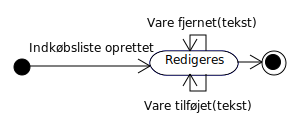
\includegraphics[scale=1]{billeder/foodl/thumbnails/indkoebsliste.png}
	\capt{Denne figur har til formål at give et overblik over systemets indkøbsliste.}
	\label{fig:overblik-indkoebsliste}
\end{figure}

Brugeren har mulighed for at tilføje varer i feltet ``tilføj til indkøbsliste'' og trykke på ``tilføj'' i bunden af siden. Der er mulighed for at slette alle varer fra indkøbslisten, ved at trykke på knappen ``slet alt'' i øverste højre hjørne af indkøbslisten, og ligeledes at slette enkelte varer, ved at trykke på de små gule krydser ud for alle varerne. Derudover er der implementeret en knap, til at udskrive indkøbslisten, som vi naturligvis kalder for ``udskriv''.

Hvis brugeren ikke er logget ind, vil de se i øverste højre hjørne af \figref{fig:overblik-indkoebsliste} (under sidehovedet) en boks, som informerer brugeren om, at man skal være logget ind for at systemet skal være i stand til at gemme indkøbslisten og favoritter. Oprettelse af bruger og indlogning bliver beskrevet nærmere i \secref{subsec:brug-opret}.

\subsection{Råvare}
Når nogen i sin husstand køber en råvare, indtræffer hændelsen \textit{råvare købt}. Denne hændelse fører råvare-klassen i en ny tilstand, der hedder \textit{brugbar}. Denne råvare er klar til at blive brugt. Inden der bliver handlet ind, og inden der sker et tilstandsskift, så er råvaren i en tidligere tilstand, der hedder \textit{eksisterer}. Dette tilstandsdiagram har ikke en afsluttendde hændelse, fordi vi har vurderet, at en råvare altid vil eksistere. Men den er først brugbar, når man har købt den. 

Indehaverne af en råvare har nu to muligheder. Man kan enten bruge hele råvaren, eller man ende med at smide noget af den ud. Disse to hændelser har vi samlet under en fælles hændelse, som vi kalder \textit{råvare opbrugt}. Denne hændelse fører klassen i en gammel tilstand, der hedder \textit{eksisterer}, da den ikke længere er brugbar i husstanden. Se \figref{fig:raavare-adfaerd}.

\begin{figure}[H]
	\centering
	\scalebox{0.8}{
	\input{billeder/tilstandsdiagrammer/raavare.pdf_tex}}
	\capt{Tilstandsdiagram for klassen råvare. De afrundede rektangulære bokse med tekst, skal anses som tilstande, som klassen kan have. De pile, der fører til en tilstand, skal anses som hændelser, som kan være skyld i et tilstandsskift. I dette tilfælde har klassen to tilstande (eksisterer) og (brugbar). Dette tilstandsdiagram har ikke en afsluttendde hændelse.}
	\label{fig:raavare-adfaerd}
\end{figure}
\subsection{Opskrift}
En opskrift kan befinde sig i en kogebog, på et stykke papir eller på en hjemmesiden. I \figref{fig:opskrift-adfaerd}, ses adfærden for klassen ``Opskrift''. En opskrift kommer til live, ved hændelsen \textit{opskrift fundet}. Her befinder den sig i tilstanden \textit{findes i opskriftssamlingen}. Hvis man er rigtig glad for en opskrift, kan man sætte et bogmærke på opskriften, så man hurtigt kan finde den igen. Sådan en hændelse kaldes for \textit{bogmærke tilføjet}. Hvis man ombestemmer sig og fjerner bogmærket, indtræffer hændelsen \textit{bogmærke fjernet}. Derudover kan man være nødsaget til at handle ind til en specifik opskrift, fordi man mangler nogle ingredienser. Det betyder, at man skal tilføje nogle opskrifter til en indkøbsliste. Denne hændelser kaldes for \textit{skrevet på indkøbsliste} med den modsignende hændelse \textit{fjernet fra indkøbsliste}. Der kan også eksistere en fejl i opskriften. En fejl kunne være et manglende billede til opskriften, eller at der står 20 minutter i ovnen i stedet for 40. Dette er beskrevet ved hjælp af hændelsen ``fejl fundet''. Disse fire hændelser medfører ikke et tilstandsskift. Opskriften ryger kun ud af tilstanden \textit{findes i opskriftssamlingen}, når opskriften fjernes, vha. hændelsen \textit{opskrift smidt ud}..

\pdffig[0.8]{tilstandsdiagrammer/opskrift}
  {Tilstandsdiagram for klassen opskrift. Klassen har én tilstand (findes i opskriftssamlingen) og en afsluttende hændelse ``opskrift fjernet'', der fører klassen ud i en sluttilstand.}
  {fig:opskrift-adfaerd}

\subsection{Bogmærke}
Som nævnt kan man vælge at tilføje et bogmærke til en opskrift, man kan lide. Denne hændelse kaldes \textit{bogmærke sat ind}, og bringer klassen i tilstanden \textit{aktiv}. Bogmærket er aktiv, indtil den kommer i sluttilstanden efter, at hændelsen \textit{bogmærke fjernet} indtræffer. Se \figref{fig:bogmaerke-adfaerd} for tilstandsdiagrammet over denne klasse.

\pdffig[0.8]{tilstandsdiagrammer/bogmaerke}
  {Tilstandsdiagram for klassen bogmærke. Klassen har én tilstand (aktiv) og en afsluttende hændelse ``bogmærke fjernet'', der fører klassen ud i sluttilstanden.}
  {fig:bogmaerke-adfaerd}

\subsection{Ingrediens}

\todo{Revider hele dette afsnit!}
En ingrediens kommer til verdenen sammen med en opskrift. Dette er fordi, at en ingrediens ikke er en del af problemområdet før den optræder i en opskrift. Det er nemlig først der, at man i en husstand behøver at bekymre sig om ingredienser. Hvis de ikke fandtes i nogle opskrifter, var der ikke nogen grund til at indkøbe en råvare svarende til ingrediensen, og ingrediensen ville derved ikke være en del af problemområdet. Denne hændelse kaldes \textit{Opskrift fundet}. Mens ingrediensen ekisister, er den i tilstanden af samme navn. Når man kender til en ingrediens, kan man skrive den på sin indkøbsliste. Dette gør man hvis man vil være sikre på at huske at købe en råvare svarende til ingrediensen, når man er ude at handle ind. Man kan selvfølgelig også fjerne ingrediensen fra sin indkøbsliste, hvis man har ombestemt sig og ikke ønsker at huskes på at købe den tilsvarende råvare. Disse to hændelser kaldes \textit{ingrediens tilføjet} og \textit{ingrediens fjernet}. Når opskriften, der indeholder en given ingrediens, smides ud, er hændelsen \textit{Opskrift smidt ud} netop indtruffet, og ingrediensen bringes i sin sluttilstand. Det bør bemærkes, at 2 forskellige opskrifter, der begge indeholder pasta, anses for at indeholde hver sin ingrediens. Dette er en vigtig adskillelse, da ingredienser består af en mængde og enhed, \fx 200 g pasta.

\begin{figure}[H]
	\centering
	\scalebox{0.6}{
	\input{billeder/tilstandsdiagrammer/ingrediens.pdf_tex}}
	\capt{Tilstandsdiagram for klassen ingrediens. I dette tilfælde har klassen én tilstand, nemlig eksisterer, og en afsluttende hændelse, der fører klassen ud i en sluttilstand.}
	\label{fig:ingrediens-adfaerd}
\end{figure}

 
\subsection{Sammendrag}
\label{sec:forbilleder:sammendrag}
De tre forbilleder: For Resten, DK-Kogebogen og Opskrifter.dk er i foregående afsnit blevet undersøgt og analyseret. Vi har i vores undersøgelse og analyse lagt vægt på fire hovedpunkter: antallet af opskrifter i systemet, Kvaliteten af opskrifterne, systemets fleksibilitet og opskriftssøgningsfunktionen (også kaldet ``Tøm køleskabet''-funktionen). De fire hovedpunkter er specificeret i detaljer i (REFERER TIL AFSNIT FORBILLEDER). For at skabe et samlet overblik, har vi valgt at samle de vigtigste og mest karakteristiske dele fra hver af forbillederne i dette afsnit.

\begin{table}
\centering
\begin{tabular}{| c | c | c | c |}
\hline
\textbf{Forbillede} & For Resten & DK-kogebogen & Opskrifter.dk \\ \hline
\textbf{Antal opskrifter} & 550 & 36.500 & 2.700 \\ \hline
\end{tabular}
\capt{Antallet af opskrifter i de tre forbilleder: For Resten, DK-Kogebogen og Opskrifter.dk. Antallet er angivet i cirkatal, da det præcise antal ikke er væsentligt.}
\label{table:forbilledeantal}
\end{table}

Som det ses i tabel (REFERER TIL TABEL HER), har DK-Kogebogen det langt største antal opskrifter, mens Opskrifter.dk har ca. fem gange flere opskrifter end For Resten. Dermed har DK-Kogenbogens ``Tøm køleskabet''-funktion også langt bedre chance for at give brugeren et resultat, når han/hun søger på opskrifter med specifikke ingredienser. Til gengæld er kvaliteten af opskrifterne på DK-Kogebogen meget varierende, og derfor kan brugeren risikere at støde på opskrifter, som er dårlige eller ubrugelige. Kvaliteten af opskrifterne på For Resten er sammenlagt dårlig. Opskrifterne er udelukkende lavet eller tilføjet af folkene bag app’en, og derfor er opskrifternes opbygning og design konsistent, hvilket naturligvis havde været en god egenskab, hvis det ikke var for det faktum, at opbygningen er uoverskuelig. Der er nemlig ingen ingrediensliste på opskriften og beskrivelsen af fremgangsmåden er også kortfattet. Derimod er kvaliteten af opskrifterne på Opskrifter.dk høj. Dette skyldes, at opskrifterne bliver gennemgået af en administrator, inden de bliver tilgængelige på Opskrifter.dk’s side, hvilket er modsat af DK-Kogebogen, hvor opskrifterne bliver tilgængelige med det samme. Desuden er Opskrifter.dk’s opskriftopbygning konsekvent i alle opskrifter, hvilket også er i modsætning til DK-Kogebogens opskrifter.

Der er stor forskel i fleksibiliteten fra forbillede til forbillede. I For Restens app, er det slet ikke muligt at op- og nedskalere portionsstørrelse, på DK-Kogebogens side er det kun muligt med nogle opskrifter, mens det på Opskrifter.dk er muligt at op- og nedskalere portionsstørrelse hver eneste opskrift. Det er en funktion som er meget brugbar, da man som bruger ikke ønsker at bruge en masse tid på selv at beregne en passende portionsstørrelse. Dette vil vi også bestræbe os på at implementere i de opskrifter der er tilgængelige på Foodl. Af sorteringsmuligheder af opskriftresultaterne, er det kun Opskrifter.dk som tilbyder denne mulighed. Her kan der sorteres efter alfabetisk orden, opskrifter med billeder, opskrifter med kød samt flere. Som en bruger på Opskrifter.dk dog pointere, mangler den sorteringsmulighed, som sortere efter de opskrifter som indeholder flest af de ingredienser som brugeren har indtastet. Denne sorteringsmulighed anses for os, som værende den mest relevante, da man som bruger er interesseret i at få anvendt så mange af ens madrester som muligt. 

De tre løsninger er vidt forskellige i deres måde at håndtere søgning på. Ud fra vores afprøvninger og observationer af løsningernes fordele og ulemper, kan vi uddrage hvilke egenskaber vi ønsker at benytte i vores eget projekt. \Fx viser den generelle utilfredshed med Forbrugerstyrelsens mobilapp For Resten, at det er vigtigt med mange opskrifter og muligheden for at vælge mere end en rest. Observationerne af For Resten og Opskrifter.dk viser også at brugergrænseflade er et vigtigt element. I disse to løsninger skal man vælge ingredienser ved at lede rundt i kategorier og i For Resten endda bevæge fingeren rundt i en cirkel for at rotere hjulene for kategorier og rester. Dette føles meget ineffektivt i forhold til at skrive navnet på ingrediensen på et tastatur. Derudover er der mellem DK-kogebogen og Opskrifter.dk en markant forskel på hvordan resultater findes. I DK-kogebogen findes kun opskrifter som inkluderer alle de indtastede ingredienser, mens Opskrifter.dk finder alle opskrifter som indeholder bare én af de valgte ingredienser. Dvs. at man med DK-kogebogen får færre resultater jo flere ingredienser man skriver, mens det med Opskrifter.dk er direkte modsat, idet antallet af resultater stiger voldsomt med antallet af ingredienser man skriver. Opskrifter.dk’s måde at gøre det på, kombineret med deres manglende sortering, giver et stor uoverskuelig mængde af resultater, hvor en stor del af disse måske kun indeholder en af de valgte ingredienser. Af dette kan man aflede at en kombination af de to må være den optimale løsning. Har man valgt få ingredienser, er man sandsynligvis interesseret i at få vist resultater som indeholder alle de ingredienser man har valgt. Har man derimod valgt mange ingredienser, er man interesseret i at få vist resultater som indeholder flest muligt af de ingredienser man har valgt.
       


\chapter{Analyse af anvendelsesområdet}
\label{chap:analyseafao}

I følgende kapitel analyseres anvendelsesområdet. Metoden tager udgangspunkt i en metode introduceret i bogen Objekt Orienteret Analyse og Design, \cite[p. ~113]{ooad}. Formålet med analysen af anvendelsesområdet, er at fastsætte kravene til \Foodl systemet og dette gøres ved først at undersøge hvilke aktører vil interagere med systemet, derefter hvordan de vil bruge systemet og til sidst fastlægge hvilke funktioner skal være tilgængelig for aktørerne.

% Anvendelsesområde
\section{Brug}
\label{sec:brug}
Denne analyse af anvendelsesområdets brug, har til formål at gøre det klart, hvilke aktører, der benytter \Foodl{}. Resultatet af analysen af aktører er en mængde aktørbeskrivelser. Resultatet af denne akvitet er brugsmønstre. Hver enkelt brugsmønster vedrører en eller flere aktører. Denne relation vises i \tableref{table:aktoertabel}. Et flueben betyder at brugsmønstret i samme række vedrører aktøren i samme kolonne.

\begin{table}
  \centering
    \begin{tabular}{ r|c c c }
  \hline
                       &    \multicolumn{3}{c}{\textbf{Brugsmønstre}}   \\ 
\textbf{Aktører}       & Bruger     & Administrator & Crawler    \\ \hline 
Søgning                & \checkmark &               &            \\ 
Favorisering           & \checkmark &               &            \\ 
Indkøbslistehåndtering & \checkmark &               &            \\ 
Login                  & \checkmark & \checkmark    &            \\ 
Fejlhåndtering         &            & \checkmark    &            \\ 
Rapportering           & \checkmark & \checkmark    &            \\ 
Crawling               &            &               & \checkmark \\
    \hline
    \end{tabular}
    \capt{Aktørtabel for Foodl.}
    \label{table:aktoertabel}
\end{table}


\subsection{Aktører}
\label{sec:aktoerer}
Vi har identificeret 3 aktører (Bruger, Administartor og Dataudtrækker), som også er vist i \tableref{table:aktoertabel}, der vil kunne interagere med \Foodl{}. Vi specificerer aktører med en beskrivelse af aktøren og om nødvendigt en eller flere eksempler på hver enkelt aktør.

Disse beskrivelser har til formål at give læseren en bedre forståelse for, hvilke egenskaber og karakterisitka en sådan aktør besidder. 


\input{indhold/2.2-analyseafanvendelsesomraade/anvendelsesomraade/brug/aktoerbeskrivelser/bruger}

\input{indhold/2.2-analyseafanvendelsesomraade/anvendelsesomraade/brug/aktoerbeskrivelser/administrator}

\input{indhold/2.2-analyseafanvendelsesomraade/anvendelsesomraade/brug/aktoerbeskrivelser/crawler}


\subsection{Brugsmønstre}
\label{subsec:brugsmoenstre}
For at beskrive hændelserne, der vedører en given aktør, modellerer vi en række brugsmønstre. Brugsmønstrene præsenteres både i form af  tilstandsdiagrammer og brugsmønsterspecifikationer. Tilstandsdiagramet giver et visuelt overblik over brugsmønsteret, hvor brugsmønsterspecifikation giver en mere detaljeret beskrivelse af brugsmønsteret.

I forbindelse med modelleringen af brugsmønstre, har vi fokuseret på, at identificere så mange brugsmønsterkandidater som muligt. Vi har benyttet denne teknik i et forsøg på at sikre, i at vi ikke har overset et vigtigt brugsmønster. Kandidaterne er valgt i forbindelse med en brainstorming, og er hver især blevet analyseret for relevans efter brainstormen. Dette har resulteret i at nogle af kandidaterne er blevet fravalgt. Der har været flere grunde til, at vi har fravalgt kandidater:

\begin{itemize}[noitemsep]
\item Brugsmønstret har ikke været en del af anvendelsesområdet
\item Brugsmønstret har været for simpelt
\item Brugsmønstret har været været en del af eller magen til et andet brugsmønstre
\end{itemize}

De fravalgte kandidater, samt begrundelsen fra fravælgelsen fremgår af \apref{ap:fravalgtebrugsmoenstre}.



\begin{table}[h]
\input{indhold/2-analyse/anvendelsesomraade/brug/brugsmoenstre/favorisering}

%Noget er fucked up med brugsmoenstrene, der burde være konverteret. Der mangler x.pdf filerne
%\begin{figure}
%\centering
%\def \svgwidth{\columnwidth}
%\input{billeder/brugsmoenstre/favorisering.pdf_tex}
%\end{figure}

\end{table}

\begin{table}[h]
\input{indhold/2-analyse/anvendelsesomraade/brug/brugsmoenstre/rapportering}
\todo{INDSÆT BILLEDE AF BRUGSMØNSTER}
\end{table}

\begin{table}[h]
\input{indhold/2-analyse/anvendelsesomraade/brug/brugsmoenstre/fejlhaandtering}
\todo{INDSÆT BILLEDE AF BRUGSMØNSTER}
\end{table}

\begin{table}[h]
\input{indhold/2-analyse/anvendelsesomraade/brug/brugsmoenstre/indkoebslistehaandtering}
\todo{INDSÆT BILLEDE AF BRUGSMØNSTER}
\end{table}

\begin{table}[h]
\input{indhold/2-analyse/anvendelsesomraade/brug/brugsmoenstre/indlogning}
\todo{INDSÆT BILLEDE AF BRUGSMØNSTER}
\end{table}

\begin{table}[h]
\input{indhold/2-analyse/anvendelsesomraade/brug/brugsmoenstre/soegning}
\todo{INDSÆT BILLEDE AF BRUGSMØNSTER}
\end{table}

\begin{table}[h]
\input{indhold/2-analyse/anvendelsesomraade/brug/brugsmoenstre/crawling}
\todo{INDSÆT BILLEDE AF BRUGSMØNSTER}
\label{table:brugmoenstre}
\end{table}


\section{Funktioner}
\label{sec:funktioner}

\section{Brugergrænseflade}
\label{sec:webapplikationen}

Som resultat af prototypeafprøvningerne med informanter, som er beskrevet i afsnittene \ref{subsec:prototype1} og \ref{subsec:prototype2} følger her en præsentation og beskrivelse af den endelige brugergrænseflade. Vi har udviklet en webapplikation, som vi har valgt at kalde \Foodl{}.

\subsection{Forside}
\label{subsec:brug-forside}

Når man taster sig ind på hjemmesiden \url{http://www.foodl.dk}, bliver man mødt af en velkomsthilsen, der meget kort beskriver hjemmesidens formål og brug, som kan ses på \figref{fig:overblik-forside}. Denne hilsen kan brugeren vælge at lukke ned. En cookie bliver gemt i browseren, så velkomsthilsnen ikke bliver vist igen, medmindre browserhistorikken bliver ryddet.

\begin{figure}[H]
	\centering
	\includegraphics[scale=1]{billeder/foodl/thumbnails/forside.png}
	\capt{Denne figur har til formål at give et overblik over systemets forside.}
	\label{fig:overblik-forside}
\end{figure}

Navnet \Foodl{} er også en del af webapplikationens logo. For at gøre det klarere for en ny bruger, hvad siden handler om, erstattede vi et O i navnet med en stor ananas, fordi det er noget, der kan spises, og sidens formål er at give folk mulighed for at genbruge deres madrester. 

På toppen af alle undersider af \Foodl{} er det muligt at tilgå sidehovedet. Her er der mulighed for at navigere tilbage til forsiden ved at klikke på den mindre version af det store logo. Derudover kan man tilgå både en indkøbsliste, der er nærmere beskrevet i \secref{subsec:brug-indkoebsliste}, og en liste af favorit-opskrifter, som brugeren selv vælger fra hjemmesiden. Favoritlisten bliver beskrevet nærmere i \secref{subsec:brug-favoritliste}. Både indkøbslisten og favoritter har et tal i parentes, der fortæller brugeren, hvor mange varer, der er i den nuværende indkøbsliste, eller hvor mange opskrifter, der er gemt under favoritter. Dette kan ses påtoppen af \figref{fig:overblik-forside}. På sidehovedet kan man også logge ind i systemet eller oprette en bruger, hvilket er forklaret nærmere i \secref{subsec:brug-opret}.

Efter brugeren føler sig tryg ved hjemmesiden og evt. har lukket velkomsthilsnen ned, så er det tid til at indtaste alle de råvarer, der ønskes brugt til madlavningen. Figur \ref{fig:foodl-soegefelt} viser, hvordan en sådan søgning foregår. Der bliver løbende indtastet bogstaver, og systemet undersøger for dele af tekststrenge, der matcher det, som bliver indtastet. Ud fra disse match gives der forslag til hvilke råvarer, man kan vælge. Man kan ikke indtaste, hvad som helst som et søgekriterie i systemet. Der er en lang række råvarer at vælge imellem. Hvis der \fx bliver indtastet kød i søgefeltet, så kommer der en liste af matchende råvarer som forslag, som man kan se på \figref{fig:foodl-soegefelt}. Der er ingen begræsning for, hvor mange råvarer, der kan indtastes som søgekriterier.

\begin{figure}[H]
	\centering
	\includegraphics[scale=0.7]{billeder/foodl/soegefelt.jpg}
	\capt{Denne figur viser systemets søgefelt.}
	\label{fig:foodl-soegefelt}
\end{figure}


For at fuldføre en søgning skal man blot trykke på ``Søg'', der er til højre for søgefeltet. Når brugeren trykker ``Søg'', så arbejder systemet på at finde alle de opskrifter, der minimum har én ingrediens, der matcher en af de indtastede råvarer. Det er efter sådan en søgning, at brugeren finder ud af, hvad der er muligt at lave ud fra de råvarer, der er til rådighed (resultatet er afgrænset til den database, man har over opskrifter).

\subsection{Resultatside}
\label{subsec:brug-resultat}

Når en søgning bliver udført, så bliver brugeren navigeret videre til søgeresultatsiden, hvor man får præsenteret en liste af opskrifter, der matcher de søgekriterier, der er blevet søgt på. Figur \ref{fig:overblik-resultat} giver et overblik over, hvordan sådan en liste kan se ud.

\begin{figure}[ht]
	\centering
	\includegraphics[scale=1]{billeder/foodl/thumbnails/soegeresultat.png}
	\capt{Denne figur har til formål at give et overblik over systemets resultatside.}
	\label{fig:overblik-resultat}
\end{figure}

I første omgang er opskrifterne sorteret efter relevans, dvs. hvor mange ingredienser, der matcher de forskellige indtastede råvaretyper. Figur \ref{fig:overblik-resultat} viser et eksempel af, hvordan sådan en liste ser ud. De ingredienser, der matcher søgekriterierne bliver markeret med fed skrift. 

På hjemmesiden vises der kun hvilke ingredienser, der skal til for at lave opskriften, men selve fremgangsmåden er ikke vist nogen steder. Man er nødt til at tilgå den oprindelige hjemmeside, hvorfra opskriften stammer fra. Dette gøres ved at trykke på enten opskriftens titel eller billedet. Begge elementer består af et link til opskriftens originale hjemmeside. 

Opskrifternes fremgangsmåde kan ikke ses på \Foodl{}, men alle andre vigtige elementer af opskriften er synlige. En opskrift består af følgende elementer:

\begin{itemize}[noitemsep]
  \item Titel
  \item Billede
  \item Vurdering
  \item Tilberedningstid
  \item Relevans (antal matchende ingredienser)
  \item Ingredienser
  \item Knapper
    \begin{itemize}[noitemsep]
      \item Tilføj alle ingredienser til indkøbsliste
      \item Tilføj / fjern fra favoritter
      \item Tilføj enkelte ingredienser til indkøbsliste
      \item Indmeld en fejl med opskriften
    \end{itemize}
\end{itemize}

Alle opskrifter består af en beskrivende titel og et relevant billede, der skal vise brugeren, hvordan opskriften kan se. Billedet er med til at vække en interesse hos brugeren og var i øvrigt ønsket fra informanterne. Tilberedningstiden er også en vigtig ting at være klar over, og denne kommer under billedet. De matchende ingredienser er markeret med fed skrift, så har brugeren nemmere ved at gennemskue, hvad der \fx er relevant at handle ind ud fra alle ingredienserne. Derudover er der et sæt knapper, som brugeren kan bruge. Se \figref{fig:foodl-opskrift}. I øverste højre hjørne er der en knap, der har et notesblok-lignende ikon. Denne knap tilføjer alle ingredienserne til indkøbslisten. Der er også mulighed for at tilføje de enkelte ingredienser ved at trykke på de små +'er ud for ingredienserne. Indkøbslisten bliver beskrevet yderligere i \secref{subsec:brug-indkoebsliste}. 
Ydermere er der mulighed for at tilføje og fjerne en opskrift til ens favoritliste. Dette gøres ved at trykke på den hjerte-formede knap. I nederste højre hjørne er der en advarselsknap, der bruges til at rapportere om eventuelle fejl ved den specifikke opskrift.

\begin{figure}[ht]
	\centering
	
\includegraphics[scale=0.7]{billeder/foodl/opskrift.jpg}
	\capt{Her ses et eksempel på en opskrift, der kan være et resultat på en søgning.}
	\label{fig:foodl-opskrift}
\end{figure}

I toppen af resultatsiden, som er vist på \figref{fig:overblik-resultat}, er der en toolbar, hvorfra brugeren har forskellige muligheder for at manipulere søgningsresultatet. Der er blevet implementeret en toolbar i toppen af siden, der følger brugerens bevægelser mht. at scrolle op og ned. På denne måde behøver brugeren ikke at scrolle helt til toppen for at udføre en handling på søgningsresultatet. 

Figur \ref{fig:foodl-toolbar} præsenterer toolbaren. I venstre side er der en samling af tre knapper, der bruges til at begrænse søgningsresultatet mht. tilberedningstiden. Her er der mulighed for at markere flere af gangen, og default kriteriet er, hvis ingen er markeret, så er alle markeret. Dette betyder, at systemet starter med at vise alle resultater. 
I midten af toolbaren er der et skaleringsværktøj, der kan bruges til at skalere opskrifternes portioner mht. antal personer. Man kan skalere dem ned til en person og op til 10 personer. Vi valgte 10 som maximum, fordi det er relativt let at skalere yderligere, hvis dette er ønsket og det er de færreste gange, man sverer rester for over 10 mennesker.
I højre side af toolbaren er der endnu en samling af tre knapper, men disse benyttes til at sortere opskrifterne. Default er ``relevans''. De to knappesamlinger er forskellige på to måder; hvad de bruges til, og at der kun er mulighed for at markere en knap af gangen ved sorteringsknapperne (højre side) og mulighed for markering af flere af gangen ved afgrænsningsknapperne (venstre side).

\begin{figure}[H]
	\centering
	\includegraphics[scale=0.7]{billeder/foodl/toolbar.jpg}
	\capt{Systemets toolbar, der er direkte under sidehovedet.}
	\label{fig:foodl-toolbar}
\end{figure}

Ud over toolbaren, så viser \figref{fig:foodl-sidebar} en sidebar, hvilket gør det muligt for brugeren at følge med i, hvad der blev søgt på, og den giver brugeren mulighed for at lave endnu en søgning. Man kan herfra slette og/eller tilføje nye råvaretyper til en ny søgning. Denne sidebar følger også med brugeres skærmrulning, da det skal være nemt og hurtigt at lave en ny søgning, hvis dette bliver aktuelt, uanset hvor mange opskrifter, der bliver vist som resultat.

\begin{figure}[H]
	\centering
	\includegraphics[scale=0.7]{billeder/foodl/sidebar.jpg}
	\capt{Systemets sidebar, der vises ved resultatsiden.}
	\label{fig:foodl-sidebar}
\end{figure}

Hvis en bruger vælger at benytte sig af indkøbslisten, så kan denne tilgås via sidehovedet, ved at trykke på ``indkøbsliste''. I sidehovedet kan man også se, hvor mange varer, der allerede er blevet tilføjet til listen.

Hvis brugere opdager en fejl med en af opskrifterne, så er det muligt at rapportere fejl i systemet. På alle opskrifterne er der en trekantet advarsels-knap i nederste højre hjørne, som kan bruges til at rapportere en fejl vedr.\ en opskrift. Figur \ref{fig:foodl-fejlrapportering} viser, hvordan det ser ud, når en bruger trykker på rapporteringsknappen ved en opskrift. Der popper en lille boks op, og baggrunden af siden bliver mørk for at fokusere koncentrationen på oprettelse af fejlrapporten. Her kan man nu specificere, hvad fejlen handler om og evt.\ give en beskrivelse, inden man vælger at indsende fejlen. Beskrivelsesfeltet vises dynamisk i forhold til den valgte fejlkategori.

\begin{figure}[H]
	\centering
	\includegraphics[scale=0.7]{billeder/foodl/fejlrapportering.jpg}
	\capt{Systemets fejlrapportering.}
	\label{fig:foodl-fejlrapportering}
\end{figure}

\subsection{Indkøbsliste}
\label{subsec:brug-indkoebsliste}

Ud over muligheden for at tilføje opskrifternes ingredienser til indkøbslisten, så kan man også tilføje almindelig tekst til, så det er muligt at lave en indkøbsliste, der indeholder andet end ingredienser til madlavningen. Så man kan skrive andre varer på, som man kan købe med fra \fx supermarkedet. Systemets indkøbsliste kan ses i \figref{fig:overblik-indkoebsliste}.

\begin{figure}[H]
	\centering
	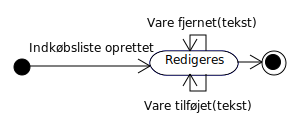
\includegraphics[scale=1]{billeder/foodl/thumbnails/indkoebsliste.png}
	\capt{Denne figur har til formål at give et overblik over systemets indkøbsliste.}
	\label{fig:overblik-indkoebsliste}
\end{figure}

Brugeren har mulighed for at tilføje varer i feltet ``tilføj til indkøbsliste'' og trykke på ``tilføj'' i bunden af siden. Der er mulighed for at slette alle varer fra indkøbslisten, ved at trykke på knappen ``slet alt'' i øverste højre hjørne af indkøbslisten, og ligeledes at slette enkelte varer, ved at trykke på de små gule krydser ud for alle varerne. Derudover er der implementeret en knap, til at udskrive indkøbslisten, som vi naturligvis kalder for ``udskriv''.

Hvis brugeren ikke er logget ind, vil de se i øverste højre hjørne af \figref{fig:overblik-indkoebsliste} (under sidehovedet) en boks, som informerer brugeren om, at man skal være logget ind for at systemet skal være i stand til at gemme indkøbslisten og favoritter. Oprettelse af bruger og indlogning bliver beskrevet nærmere i \secref{subsec:brug-opret}.

\subsection{Favoritliste}
\label{subsec:brug-favoritliste}

Når der bliver tilføjet en opskrift til en brugers favoritliste, så kan denne opskrift findes under ``favoritter'', som kan findes via sidehovedet i toppen af siden. Et eksempel af en kort opskriftsliste under favoritter kan ses på \figref{fig:overblik-favoritter}.

\begin{figure}[H]
	\centering
	\includegraphics[scale=1]{billeder/foodl/thumbnails/favoritter.png}
	\capt{Denne figur har til formål at give et overblik over systemets favoritside.}
	\label{fig:overblik-favoritter}
\end{figure}

En opskrift bliver tilføjet til favoritlisten ved at trykke på den hjerte-formede knap i øverste højre hjørne af en opskrift. Hvis en opskrift ikke er favoriseret, så er det hjerteformede område i knappen gråt. Når den bliver favoriseret, så bliver hjertet rødt, og dette kan ses i \figref{fig:overblik-favoritter}.

Idéen med favoritlisten er at give brugerne mulighed for at gemme opskrifter, de finder interessante og at de gerne vil bogmærke den til næste gang. De er meget nemmere at finde frem, når man kan finde dem under favoritlisten i stedet for at skulle udføre en ny søgning og prøve at finde den samme opskrift igen.

\subsection{Brugeroprettelse}
\label{subsec:brug-opret}

Alle har mulighed for at oprette en bruger på \Foodl{}. Hvis man har en bruger og logger ind på systemet, så kan man kan gemme sin indkøbsliste og listen over favoritter. Det er dog ikke obligatorisk at have en bruger for at kunne bruge systemet, da vi ikke ønsker at binde brugerne til at oprette noget som helst. Man kan bruge hele systemet, om man har en bruger eller ej.

Man opretter en bruger på samme side, hvor man logger ind på systemet. Dette er præsenteret i \figref{fig:overblik-brugeroprettelse}. Man navigerer til denne side ved at klikke på ``log ind / opret bruger'' i højre side af sidehovedet, som også er synlig på samme figur.

\begin{figure}[H]
	\centering
	\includegraphics[scale=0.4]{billeder/foodl/thumbnails/opretbrugeroglogind.png}
	\capt{Denne figur har til formål at give et overblik over systemets brugeroprettelsesside.}
	\label{fig:overblik-brugeroprettelse}
\end{figure}

Man skal bruge sin email og en adgangskode for at lave en bruger. Hvis man allerede har en bruger, så skal man blot logge ind med de rigtige oplysninger.

Når man er logget ind, så ændrer sidehovedet sig en smule. Figur \ref{fig:foodl-loggetind} viser, at der nu er mulighed for at gå ind i en menu, der hedder ``indstillinger'' og at logge ud igen. Man kan også se, at der pludselig er indlæst en liste af favoritter på 10 opskrifter fra tidligere et besøg.

\begin{figure}[H]
	\centering
	\includegraphics[scale=0.4]{billeder/foodl/header-login.png}
	\capt{Det ændrede sidehovede, når brugeren er logget ind.}
	\label{fig:foodl-loggetind}
\end{figure}

Hvis man ønsker at skifte sin adgangskode, så sker det ved at trykke på knappen ``indstillinger'' i sidehovedet.

\subsection{Generelt}
Som de fleste andre hjemmesider, så har vi også en ``om'' og en ``kontakt'' side, som kan tilgås fra nederste venstre hjørne af enhver underside af \Foodl{}. Derudover kan man rapportere en generel fejl ved siden, hvis man støder på sådan en. Figur \ref{fig:foodl-formaliteter} viser disse tre knapper.

\begin{figure}[H]
	\centering
	\includegraphics[scale=0.7]{billeder/foodl/formaliteter.jpg}
	\capt{I nederste venstre hjørne af systemet kan man rapportere en generel fejl, læse mere om systemet og kontakte udviklerne.}
	\label{fig:foodl-formaliteter}
\end{figure}

Under ``om foodl'' kan brugeren kort læse om dette projekt og om udviklerne bag systemet, altså denne gruppe.

\subsection{Designovervejelser}
\label{subsec:designovervejelser}

\todo{DEB!}

\section{Design}
\label{chap:design}


\chapter{Implementering}
\label{chap:implementering}

\section{Ruby On Rails}
I følgende afsnit, vil vi kort beskrive Ruby on Rails, som er et open-source framework til udvikling af web-applikationer, som vores system bygger på. Vi vil desuden forklarer Model-View-Controller arkitekturen, som er den arkitektur alle Ruby on Rails applikationer tager udgangspunkt i.  

Ruby on Rails (RoR) blev udviklet i 2003 af David Heinemeier Hansson(xxx KILDE xxx), og er et forholdsvist nyt web-applikationens framework, set i forhold til eksempelvis PHP, Java og .NET(xxx KILDE xxx). David Heinemeier Hanssons intentioner med RoR var, at skabe et framework, som gjorde det lettere og hurtigere for web-programmører at udvikle webapplikationer, hvilket også er en af de væsentlige åresager til at vi valgte at anvende det. Dette gjorde han bl.a. ved at implementere filosofien: {\emph{``konventioner over konfigurationer''}(xxx KILDE xxx) i RoR. Filosofien har både sine fordele og ulemper. Det er en ulempe, at web-udvikleren skal have arbejdet med RoR i lang tid, for at kunne huske de mange konventionerne; eller bruge en masse tid, på at slå dem op. Det er på den anden siden en fordel at web-udviklere, ved hjælp af RoR's konventioner, kan lave applikationer, som kan udrette meget, ud fra få linjer kode. RoR viser allerede fra første møde, når man genererer en ny web-applikation, at der skal meget lidt arbejde til, at få et stort afkast. Dette kan ses i billede \figref{fig:Rails-new-foodl}, hvor en enkelt linje i kommandopromten, generere en ny mappe, som indeholder en fuldtfungerende Ruby on Rails web-applikation, kaldet ``Foodl''. Mappen med web-applikationen består af en lang række undermapper. Heriblandt ``App'', hvori ``models'', ``views'' og ``controllers'' befinder sig; ``Config'', hvori ``routes'' befinder sig, som er det element der forbinder controllers og views (mere om dette i følgende sektion \cite{MVC}); og undermappen ``Spec'', hvori unit testing af Models, Views og Controllers foregår; samt flere. Kort sagt genererer rails, vha. new-kommandoen, hele skelettet for web-applikationen, og derefter er det ``bare'' at fylde det indhold man ønsker i sin web-applikation, i de rigtige mapper. Ønskes der yderligere information om Ruby on Rails, og sammenspillet mellem Rails og Ruby, henvises til \cite{RoR.org}.

\begin{figure}
\centering
\includegraphics[scale=0.6]{billeder/Rails-new-foodl.png}
\capt{Railskommando, der indtastes i kommandopromten, hvorefter rails genererer en mappe med en fuldtfungerende web-applikation, kaldet ``Foodl''}
\label{fig:Rails-new-foodl}
\end{figure}

\subsection{Model-View-Controller}
\label{MVC}
Model-View-Controller (MVC) er den arkitektur en hver Ruby on Rails applikation tager udgangspunkt i. Så snart en ny Ruby on Rails web-applikation bliver genereret, vil den indeholder mapperne ``models'',``views'' og ``controllers'', så på den måde er en RoR applikation tvunget til at implementere MVC-arkitekturen. Arkitekturen blev opfundet af Trygve Reenskaug i 1979, som en slags standard arkitektur for interaktive applikationer (eksempelvis web-applikationer). Arkitekturen består af tre komponenter, nemlig modeller, views og controllers, der hverisær har nogle specifikke egenskaber og opgaver. Modellen den komponent, der har ansvaret for at applikationen 

\chapter{Kvalitetssikring}
\label{chap:kvalitetssikring}

\section{Modultest}
\label{sec:unittests}
For at verificere at programmet opfører sig som vi ønsker, har vi benyttet RSpec, hvilket er et Ruby modultestframework (unit testing framework), der først og fremmest er minded mod ``behaviour-driven development'', men også kan bruges til at skrive modultests med. Vi har modultestet bruger-modellen, fordi den er central for systemet, og den er i direkte kontakt med brugeren og kan have kritiske fejl. Derudover har vi også modultestet enkelte forespørgelser (requests i RSpec), der simulerer en brugeres interaktion med systemet. \Fx testes der login-systemet samt det HTML, der vises, efter man har logget ind. Vi har ikke foretaget modultest af hele systemet, hvilket er grundet nød af ressourcer. Idet pålidelighedskriteriet, specificeret i \chapref{chap:design}, er blevet vurderet som ``mindre vigtigt'', har vi valgt at nedprioritere dem. Eksempler på nogle af de modultest vi har foretaget på bruger-modellen, ved hjælp af RSpec, ses i \lstref{lst:password} og \lstref{lst:email}. For resten af tests refereres der til kildekoden.


Det skal nævnes, at ``@user'' er en instansvariabel defineret tidligere i modultestfilen og er et objekt af klassen ``user'' (se \secref{sec:modelfunktion}), der indeholder de attributter og metoder, der hører med til alle instanser af klassen. Eksempel \ref{lst:password} viser en enkel modultest for brugeroprettelsesprocessen. Her skal kodeordfeltet og kodeordbekræftelsesfeltet være præcis ens, ellers kan objektet ikke være valid. Metoden \methodref{valid?} på bruger-objektet er en Active Record metode (bruger-modellen nedarver fra ActiveRecord-klassen) og returnerer blot sand eller falsk, alt afhængigt om objektet kan gemmes i databasen eller ej. Denne metode bliver kaldt på linje 3 i eksemplet.

\begin{lstlisting}[caption={Modultest af brugerens har indtastede password, når han/hun opretter sig som bruger},label=lst:password,language=Ruby]
describe "when password is not present" do
  before { @user.password = @user.password_confirmation = " " }
  it { should_not be_valid }
end
\end{lstlisting}

Eksempel \ref{lst:email} viser modultest af emailadressefeltet, også fundet i brugermodellen. Her testes der på validiteten af emailadressen. Emailadresser i bruger-modellen bliver tjekket af et regulære udtryk, inden objektet gemmes i databasen. Derfor testes der på adresser, der strider imod det regulære udtryk og burde derfor ikke godkendes ved brug af \methodref{@user.valid?}.

\begin{lstlisting}[caption={Modultest af en brugers email er valid, når han/hun opretter sig som bruger},label=lst:email,language=Ruby]
describe "when email format is invalid" do
  it "should be invalid" do
    addresses = %w[user@foo,com user_at_foo.org example.user@foo.
                   foo@bar_baz.com foo@bar+baz.com]
    addresses.each do |invalid_address|
      @user.email = invalid_address
      @user.should_not be_valid
    end
  end
end
\end{lstlisting}

Der er foretaget flere lignende modultest på bruger-modellen samt login-systemet. Der er ikke nogen konkret kodedækningsprocent, da det er svært at vurdere, hvorvidt de forskellige actions er blevet testet.

\subsection{Metode til at finde lighed mellem tekststrenge}
Vi benyttede en ret simpel fremgangsmåde til at modulteste metoden \methodref{CompareStrings}, der tester ligheden mellem to tekststrenge. Vi testede denne funktion i Ruby, ved at initialisere et array som vist i \lstref{lst:testcases}. Der er ikke brugt RSpec til modultest af dette program.

\begin{lstlisting}[caption={Et eksempel på en række testcases til brug ved modultest.},label=lst:testcases,language=Ruby]
test_cases = [
  ["aa12345", "aa67890", "aa"],
  ["aa12345", "678aa90", "aa"],
  ["aa12345", "67890aa", "aa"]
]
\end{lstlisting}

I arrayet \texttt{test\_cases}, består hvert element af et array, hvor hvert element i nævnte rækkefølge er: [input1, input2, forventet returværdi].
For hvert element i arrayet, blev det testet om \methodref{CompareStrings(input1, input2)} returnerede den forventede værdi. Eksemplet er kun et udpluk af 26 test-cases, der fremgår af kildekoden.

\chapter{Konklusion}
\label{chap:konklusion}
%Problemformulering
%Opfyldelse af kriterier
%Implementering
%Informanternes inddragelse og samarbejde

I vores projektforløb har vi arbejdet med at løse et problem, som i problemformuleringen blev beskrevet som følger:

``Hvordan kan man, vha. et system, øge brugen af madrester i madlavningen i danske husstande?''

Til at løse problemet, udviklede vi en web-applikation, kaldet \Foodl{} (\url{http://foodl.dk}), som ved hjælp af indtastning af nogle ingredienser og madvarer, kommer med forslag til relevante opskrifter. Med relevante, menes opskrifter, som indeholder så mange af de indtastede ingredienser og madvarer som muligt, så disse kan blive anvendt.

Hvordan \Foodl{} fungerer på det tekniske niveau, er beskrevet i kapitel 6, kaldet Implementering \ref{chap:implementering}. Til udvikling af systemet, anvendte vi en objektorienteret metode fra bogen ``Objekt Orienteret Analyse \& Design'' \cite{ooad}. Metoden er meget anvendelig i forhold til at analysere og designe objektorienterede systemer, som eksempelvis web-applikationer. 

Hvordan \Foodl{} fungerer på det tekniske niveau, er bekskrevet i \chapref{chap:implementering}, implementering. Til udvikling af systemet, anvendte vi en objektorienteret metode fra bogen ``Objekt Orienteret Analyse \& Design'' \cite{ooad}. Metoden er meget anvendelig i forhold til at analysere og designe objektorienterede systemer, som eksempelvis web-applikationer. 

I projektforløbet har vi haft et tæt samarbejde med to informanter, Merete og Keld. Sammen med informanterne, formulerede vi en systemdefinition, som kan ses i \chapref{chap:systemvalg}, \secref{subsec:alternativesystemdefinitioner}. Systemdefinitionen opfylder BATOFF-modellens punkter, som beskriver hvad systemet skal kunne, hvor det skal kunne tilgåes fra, under hvilke forhold systemet bliver lavet, mm. Vi konkludere, at \Foodl{} lever op til systemdefinitionen, og at det, ved hjælp af \Foodl{}, er blevet lettere for danskerne, at få inspiration til, hvordan de kan få anvendt deres madrester.

Samarbejdet med informanterne omfatter møder, som har hjulpet os med, at blive mere bevidste om, hvilke kriterier systemet skulle opfylde, for at blive så attraktiv som muligt. Samarbejdet har desuden omfattet test af systemet ved hjælp af prototyper og en usability test af det endelige system. Ved brug af protoyper, blev vi mere bevidste om, hvordan \Foodl{}'s brugergrænseflade skulle opstilles, for at være brugbar, samt helt konkret, hvilke funktioner systemet skulle indeholde.

Alt det analyserede er blevet designet. Af det designede, er der dog ting vi ikke har valgt at implementere af hensyn til deadline for projektet:
\begin{itemize}
\item Dataudtrækkeren gennemgår kun opskriftssiderne på Arla én gang. Der er ikke implementeret muligheden for at vende tilbage til disse sider og tjekke om der er sket ændringer, for i givet fald at opdatere modellen.
\item Fejlrapportering af opskrifter er kun delvist implementeret. Man kan rapportere fejl i en opskrift fra søgesiden ud fra den opskrift, der er fejl i. Den generelle fejlrapporteringsknap, der findes som en footer på alle sider har dog ingen funktion.
\end{itemize}


\section{Perspektivering}
\label{chap:perspektivering}




\cleardoublepage
	
\bibliographystyle{plain}
\bibliography{kildeliste}

\part{Akademisk rapport}


\part{Bilag}

\appendix

%\chapter{Appendiks Eksempel}
\label{ap:eksempel}

\chapter{Fravalgte klasser}
\label{ap:fravalgteklasser}

Herunder ses de fravalgte klasser, som gruppen ikke finder relevante i forhold til problemområdet. De listes her, da der har været meget diskussion, om hvorvidt klasserne skulle med i systemet eller ej. 

\begin{description}
\item[Person] \hfill \\
Vi vælger at fjerne person-klassen, fordi vi mener, at vores løsning ikke skal være noget socialt media, og derfor mener vi, at det er selve husholdningen, der er fælles om madlavningen selvom det måske blot er en person, der laver mad og står for indkøb og lignende. Brugeren af programmet er ikke en del af problemområdet og skal derfor ikke modelleres som klasse.

\item[Køkken] \hfill \\
Køkken og husholdning dækker over samme del af problemområdet, og vi fjerner derfor køkken og vurderer bagefter om husholdning skal være en klasse.

\item[Husholdning] \hfill \\
En husholdning repræsenterer et hjem, som indeholder én til flere personer. Det er ikke en del af problemområdet at holde styr på eller at kommunikere med andre husstande.

\item[Køleskab/skab/opbevaringsskab] \hfill \\
Om råvarene befinder sig i et køleskab eller i en skuffe er, for os, uinteressant, derfor er vi ikke interesseret i at modellere disse skabe som en klasse.

\item[Køkkenredskab/komfur] \hfill \\
Ligesom ved køleskab/anden opbevaring er vi ikke interesseret i at modellere hvilke redskaber husholdningen har adgang til.

\item[Service] \hfill \\ 
Vi har valgt at fjerne klassen service, fordi denne ikke findes i vores problemområde. Service er noget, der bliver brugt, når man er i færd med at spise det færdige mad, og ikke under selve madlavningen.

\item[Butik] \hfill \\
Vi har valgt at fjerne klassen Butik, da vores system fokuserer på madspild og varieret kost. En modellering af butikker ville være relevant, hvis vores fokus lå på at begrænse udgifter på mad, men da dette imidlertidig ikke er situationen i problemområdet, bliver den udeladt.

\item[Typisk/atypisk ingrediens] \hfill \\
Det er ikke en del af problemområdet at folk ikke er klar over hvilke ingredienser der er normale/unormale at have.

\item[Enhed/Mængde] \hfill \\
Enhed og mængde er ikke klasser, men attributter til en ingrediens.

\item[Madplan] \hfill \\
Informanterne syntes ikke at en madplan var særlig nødvendig. Den indgik i systemdefinition S2, som informanterne fravalgte. Madplanen anses derfor som overflødig, hvorfor denne fjernes som klasse.
\end{description}




\end{document}
